\chapter{Image Processing}
\label{chap:image_processing}

\begin{figure}[ht]
	\hfill
	\begin{minipage}{0.5\textwidth}
		\centering
		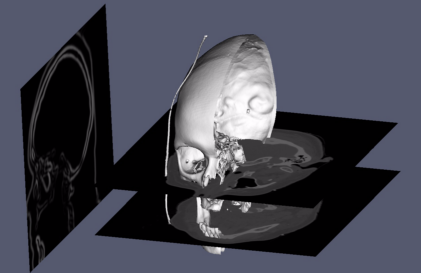
\includegraphics{VTKTextbook-216}
		\caption*{\texttt{Gradient magnitude of a slice (vertical) of the Visible Woman CT dataset shown with an isosurface and two slices (horizontal) of the dataset.}}
	\end{minipage}
\end{figure}

\firstletter{I}n this chapter we describe the image processing components of the Visualization Toolkit.
The focus is on key representational ideas, pipeline issues such as data streaming, and useful algorithms for improving the appearance and effectiveness of image data visualizations.

\section{Introduction}
Image processing has been a mainstay of computing since the advent of the digital computer. Early efforts focused on improving image content for human interpretation.
